% !TeX spellcheck = cs_CZ
%{\tikzset{external/prefix={tikz/FYZII/}}
% \tikzset{external/figure name/.add={ch38_}{}}
%---------------------------------------------------------------------------------------------------
% file fey2ch38.tex
%---------------------------------------------------------------------------------------------------
%=========================== Kapitola Pružnost =====================================================
\setchaptertoc
\chapter{Pružnost}\label{fyz:IIchapIIXL}

  \section{Hookeův zákon}\label{fyz:IIchapIIXLsecI}
  \section{Homogenní deformace}\label{fyz:IIchapIIXLsecII}
  \section{Torzní tyč. Střižné vlny}\label{fyz:IIchapIIXLsecIII}
  \section{Prohnutý nosník}\label{fyz:IIchapIIXLsecIV}
  \section{Vzpěrnost}\label{fyz:IIchapIIXLsecV}
  \section{Příklady a cvičení}\label{fyz:IIchapIIXLsecVI}
  

    \begin{figure}[ht!] %\ref{fyz:fig799}
      \centering
      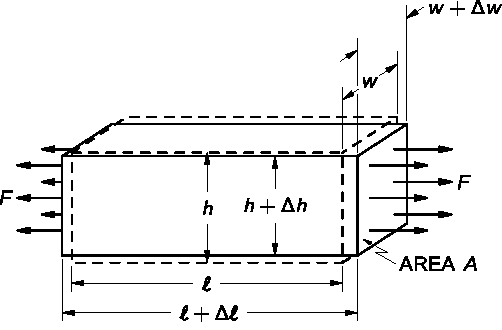
\includegraphics[width=0.7\linewidth]{fyz_fig799.pdf}
      \caption{
               (\cite[s.~707]{Feynman02})}
      \label{fyz:fig799}
    \end{figure}
    
    \begin{figure}[ht!] %\ref{fyz:fig800}
      \centering
      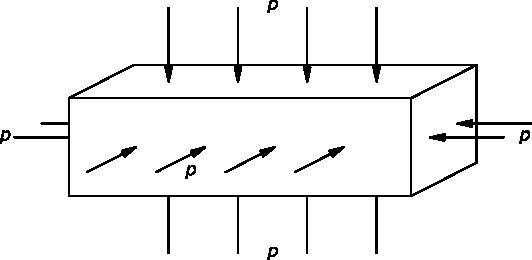
\includegraphics[width=0.7\linewidth]{fyz_fig800.pdf}
      \caption{
               (\cite[s.~707]{Feynman02})}
      \label{fyz:fig800}
    \end{figure}

    \begin{figure}[ht!]
      \centering
      \subcaptionbox{\label{fyz:fig801a}}{\luafigure[0.9]{fyz_fig801a.pdf}}               \\
      \subcaptionbox{\label{fyz:fig801b}}{\luafigure[0.9]{fyz_fig801b.pdf}}               \\
      \subcaptionbox{\label{fyz:fig801c}}{\luafigure[0.9]{fyz_fig801c.pdf}}
      \caption{
               (\cite[s.~748]{Feynman02})}
      \label{fyz:fig801}
    \end{figure}

    \begin{figure}[ht!] %\ref{fyz:fig802}
      \centering
      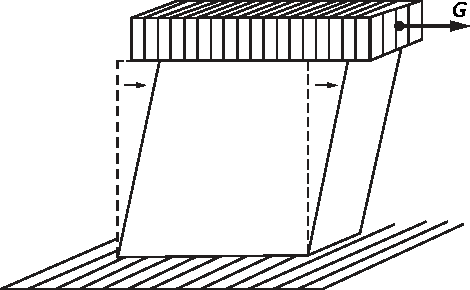
\includegraphics[width=0.7\linewidth]{fyz_fig802.pdf}
      \caption{
               (\cite[s.~707]{Feynman02})}
      \label{fyz:fig802}
    \end{figure}
    
    \begin{figure}[ht!] %\ref{fyz:fig803}
      \centering
      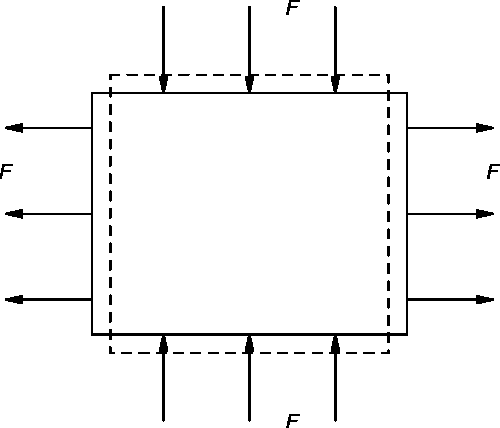
\includegraphics[width=0.7\linewidth]{fyz_fig803.pdf}
      \caption{
               (\cite[s.~707]{Feynman02})}
      \label{fyz:fig803}
    \end{figure}

    \begin{figure}[ht!] %\ref{fyz:fig804}
      \centering
      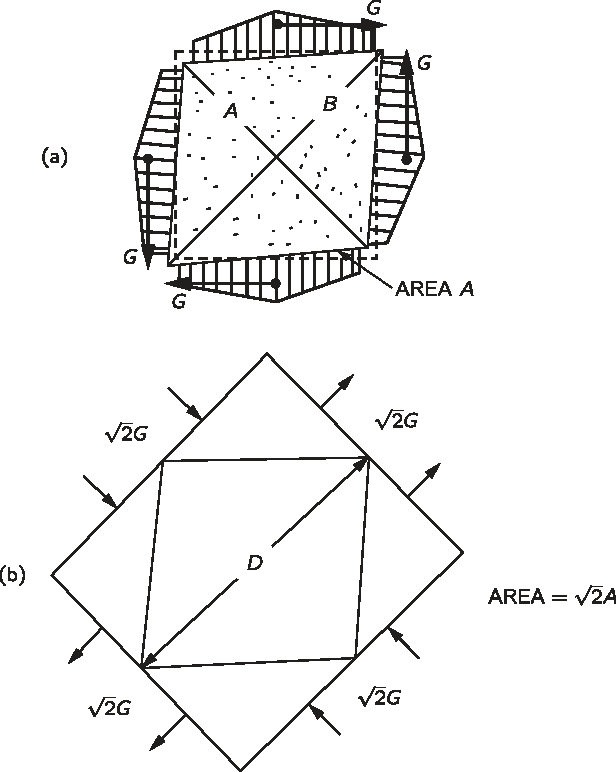
\includegraphics[width=0.7\linewidth]{fyz_fig804.pdf}
      \caption{
               (\cite[s.~707]{Feynman02})}
      \label{fyz:fig804}
    \end{figure}
    
    \begin{figure}[ht!] %\ref{fyz:fig805}
      \centering
      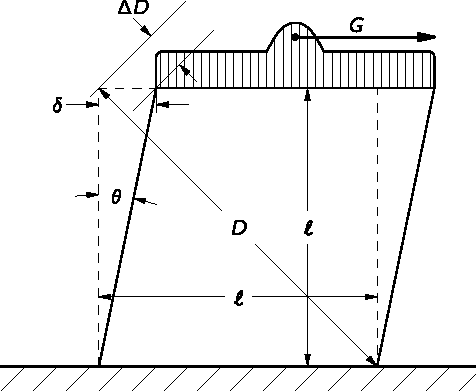
\includegraphics[width=0.7\linewidth]{fyz_fig805.pdf}
      \caption{
               (\cite[s.~707]{Feynman02})}
      \label{fyz:fig805}
    \end{figure}


    \begin{figure}[ht!] %\ref{fyz:fig806}
      \centering
      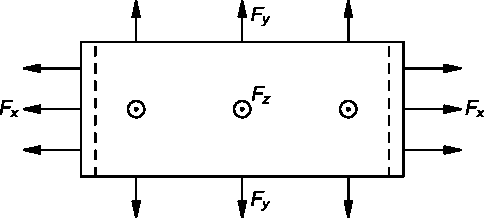
\includegraphics[width=0.7\linewidth]{fyz_fig806.pdf}
      \caption{
               (\cite[s.~707]{Feynman02})}
      \label{fyz:fig806}
    \end{figure}

    \begin{figure}[ht!] %\ref{fyz:fig807}
      \centering
      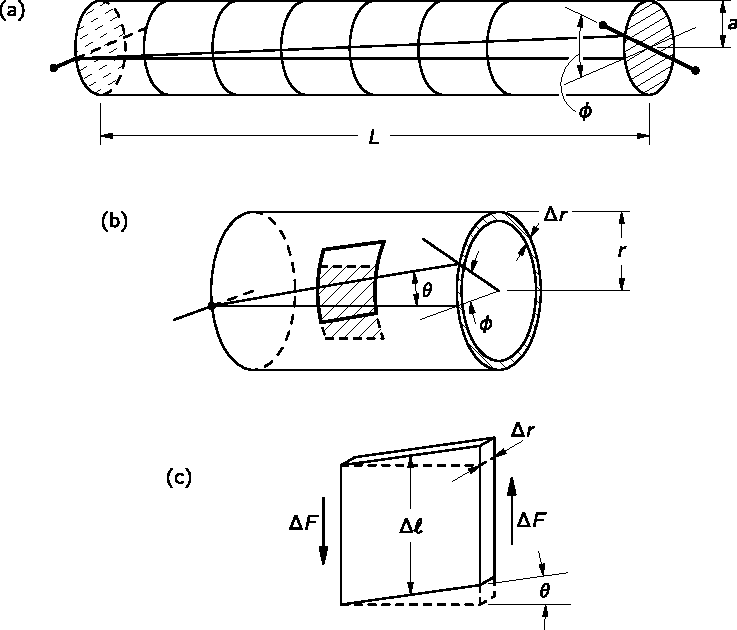
\includegraphics[width=0.7\linewidth]{fyz_fig807.pdf}
      \caption{
               (\cite[s.~707]{Feynman02})}
      \label{fyz:fig807}
    \end{figure}
    
    \begin{figure}[ht!] %\ref{fyz:fig808}
      \centering
      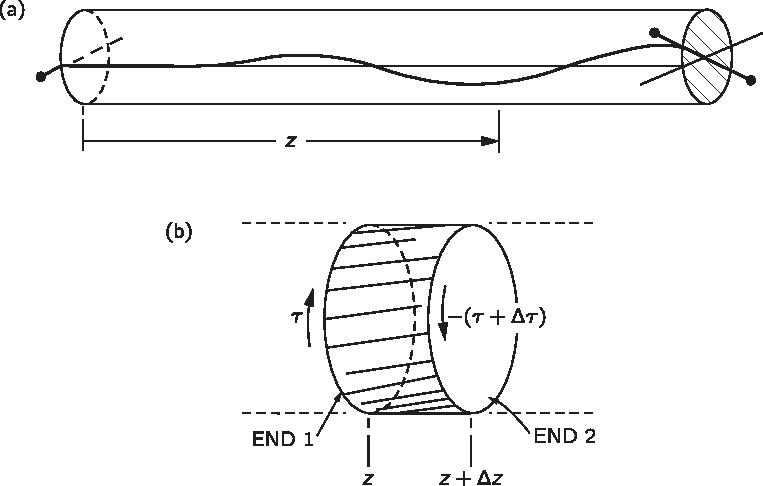
\includegraphics[width=0.7\linewidth]{fyz_fig808.pdf}
      \caption{
               (\cite[s.~707]{Feynman02})}
      \label{fyz:fig808}
    \end{figure}

    \begin{figure}[ht!] %\ref{fyz:fig809}
      \centering
      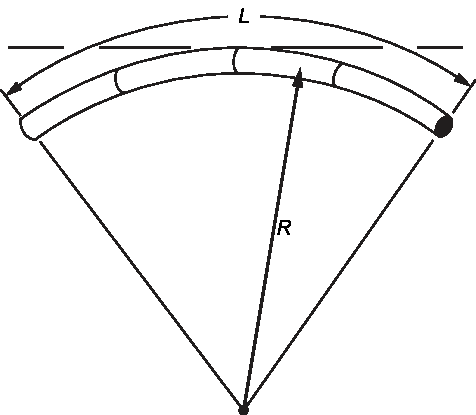
\includegraphics[width=0.7\linewidth]{fyz_fig809.pdf}
      \caption{
               (\cite[s.~707]{Feynman02})}
      \label{fyz:fig809}
    \end{figure}
    
    \begin{figure}[ht!] %\ref{fyz:fig810}
      \centering
      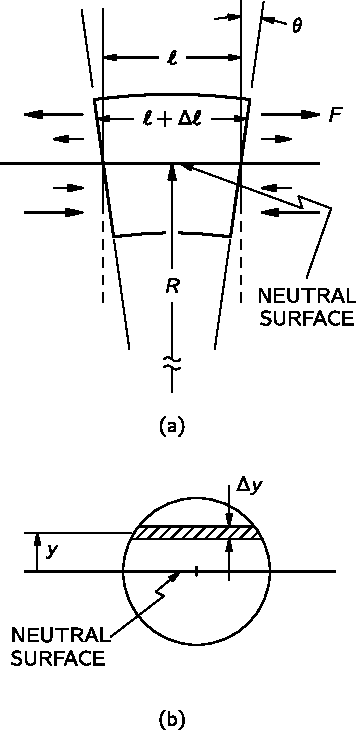
\includegraphics[width=0.7\linewidth]{fyz_fig810.pdf}
      \caption{
               (\cite[s.~707]{Feynman02})}
      \label{fyz:fig810}
    \end{figure}


    \begin{figure}[ht!] %\ref{fyz:fig811}
      \centering
      
\includegraphics[width=0.7\linewidth]{fyz_fig811.pdf}
      \caption{
               (\cite[s.~707]{Feynman02})}
      \label{fyz:fig811}
    \end{figure}

    \begin{figure}[ht!] %\ref{fyz:fig812}
      \centering
      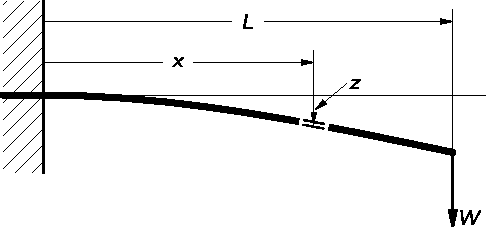
\includegraphics[width=0.7\linewidth]{fyz_fig812.pdf}
      \caption{
               (\cite[s.~707]{Feynman02})}
      \label{fyz:fig812}
    \end{figure}
    
    \begin{figure}[ht!] %\ref{fyz:fig813}
      \centering
      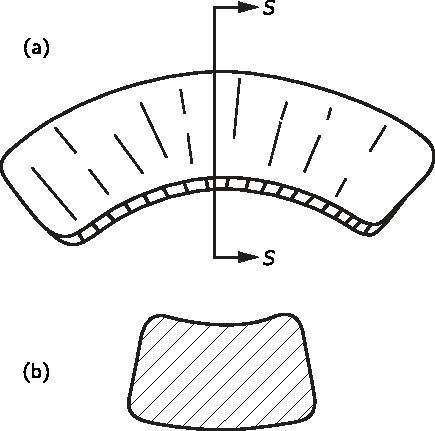
\includegraphics[width=0.7\linewidth]{fyz_fig813.pdf}
      \caption{
               (\cite[s.~707]{Feynman02})}
      \label{fyz:fig813}
    \end{figure}

    \begin{figure}[ht!] %\ref{fyz:fig814}
      \centering
      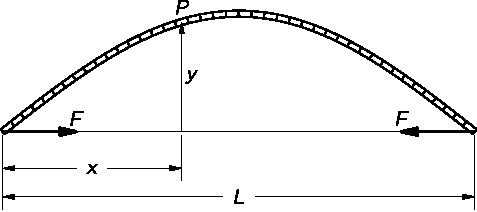
\includegraphics[width=0.7\linewidth]{fyz_fig814.pdf}
      \caption{
               (\cite[s.~707]{Feynman02})}
      \label{fyz:fig814}
    \end{figure}
    
    \begin{figure}[ht!] %\ref{fyz:fig815}
      \centering
      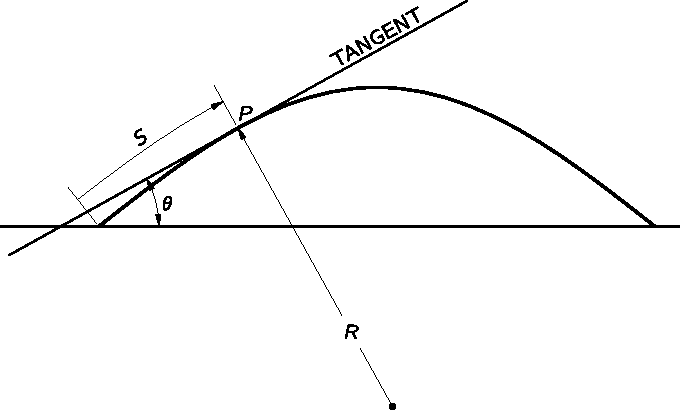
\includegraphics[width=0.7\linewidth]{fyz_fig815.pdf}
      \caption{
               (\cite[s.~707]{Feynman02})}
      \label{fyz:fig815}
    \end{figure}


    \begin{figure}[ht!] %\ref{fyz:fig816}
      \centering
      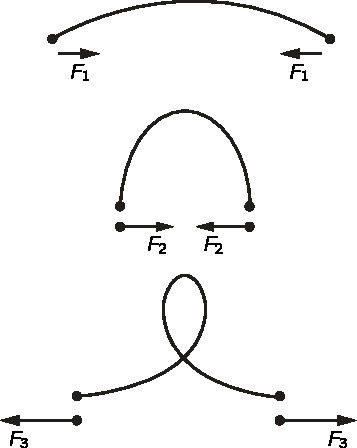
\includegraphics[width=0.7\linewidth]{fyz_fig816.pdf}
      \caption{
               (\cite[s.~707]{Feynman02})}
      \label{fyz:fig816}
    \end{figure}

    \todo[inline]{Kapitola fey2ch38 je nedodělaná, obsahuje pouze obrázky}

%} %tikzset
%---------------------------------------------------------------------------------------------------
